% !TeX spellcheck = da_DK
\subsection{Referencespænding til feedback}\label{subsec:Spaendingsref_Komparator}
\subsubsection{Teori og design}
Feedbackkonfigurationen skal forsynes med en konstant spænding, da denne skal anvendes som sammenligningsgrundlag ift. inputsignalet. Her anvendes igen en referencespænding, jævnfør afsnit \ref{subsec:Spaendingsref} på side \pageref{subsec:Spaendingsref}. Der anvendes en tilsvarende referencediode til denne referencespænding, som kan ses på \figref{fig:Spaendingsreference}, side \pageref{subsec:Spaendingsref}. \\
For at udregne modstanden R1 for referencespændingen til komparatoren benyttes \eqref{eq:udregning_modstand}, side \pageref{eq:udregning_modstand}. Den ønskede referenceværdi er $2.5$V, så der skal i dette tilfælde ikke benyttes en spændingsdeler, da disse indgår i designet for feedbackkonfigurationen. I starten af kredsløbet indsættes operationsforstærkeren af typen TL$082$, som har to inputs og outputs. \cite{Corporation2013} Den kan denne fungere som buffer til feedbackkonfigurationen og en inverterende forstærker. \cite{Schaumann2014} Den maksimale biasstrøm er $50$nA, da spændingen går direkte ind i bufferen. Biasstrømmen for referencedioden er sat til $200\mu$A. Dermed kan værdierne indsættes i formlen og R$1$ kan beregnes:
\begin{equation}
R1 = \frac{5.5V-2.5V}{50nA + 200\mu\text{A}} = 14999.62501\Omega \approx 15K\Omega 
\end{equation} 
Operationsforstærkeren benyttes, som nævnt, som en buffer og inverterende forstærker, da der både ønskes et positivt og negativt output til tærskelværdierne i feedbackkonfigurationen.
\begin{figure}[H]
	\centering
	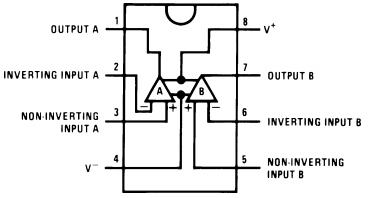
\includegraphics[scale=0.8]{figures/cProblemloesning/TL082.PNG}
	\caption{På figuren ses pinkonfigurationen af operationsforstærkeren, TL$082$. Det positive output til feedbackkonfigurationen vil komme fra pin $1$ dvs. output A, og det negative output til komparatorblokken vil komme fra pin $7$ dvs. output B. \cite{Corporation2013}}
	\label{fig:TL082}
\end{figure}
\noindent Der vides fra teorien, at der skal benyttes to modstande til designet af en inverterende forstærker. Da der ønskes et gain på 1, skal disse to modstande have samme værdi. \cite{Nilsson2011} Designet af referencespændingen med operationsforstærkeren fremgår af \figref{fig:ref_komparator}.

\begin{figure}[H]
	\centering
	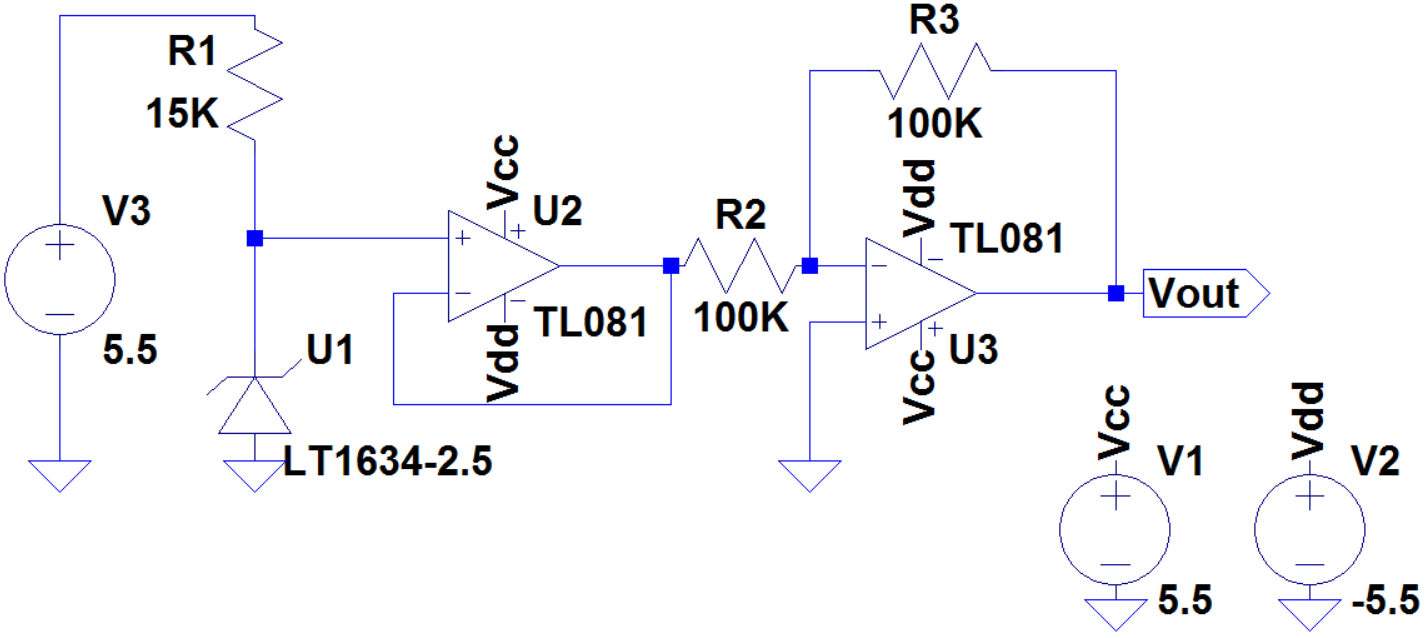
\includegraphics[scale=0.4]{figures/cProblemloesning/Reference_komparator.PNG}
	\caption{På figuren ses designet af referencespændingsblokken, der skal levere en referencespænding til feedbackkonfigurationen. Operationsforstærkeren TL$082$ fungerer som to TL$081$'ere, og derfor er simuleringen opbygget således. \cite{Corporation2013}}
	\label{fig:ref_komparator}
\end{figure}

\subsubsection{Simulering}
Der foretages en simulering i LTspice for at undersøge, hvorvidt designet fungerer ideelt og præcisionen af spændingsreferencen. På \figref{fig:Spaendingsreference_komparator_sim} ses simuleringen af spændingsreferencen og operationsforstærkeren.
\begin{figure}[H]
	\centering
	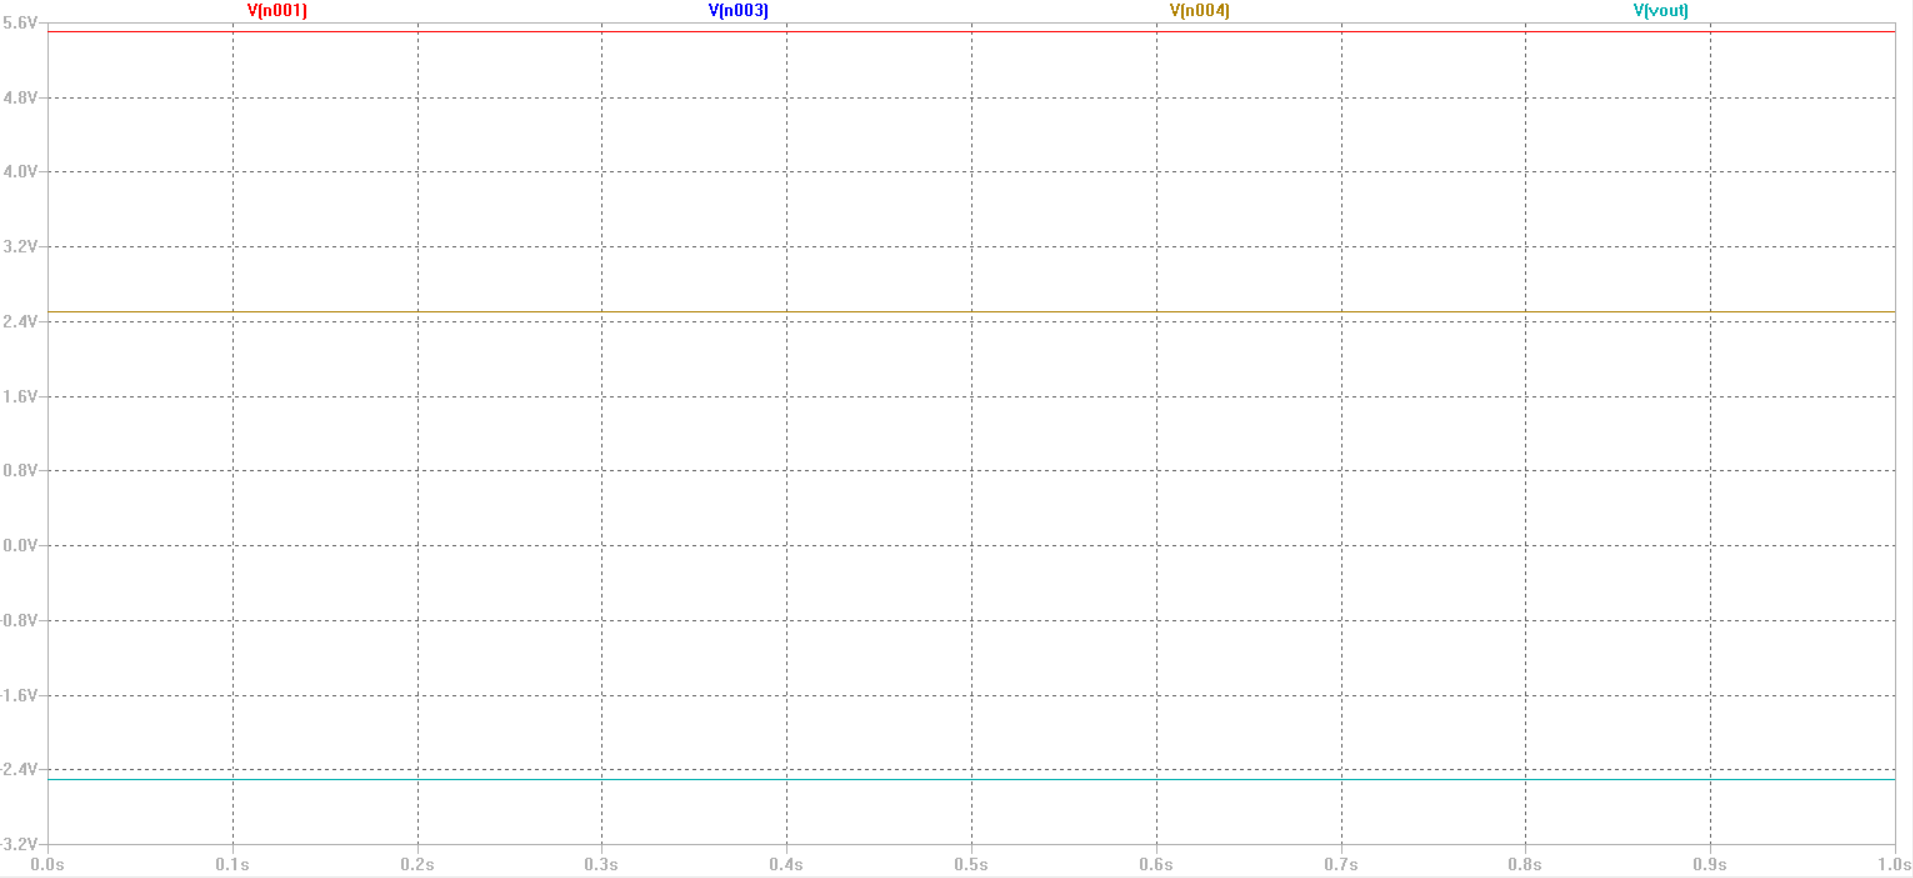
\includegraphics[scale=.36]{figures/cProblemloesning/Reference_sim_kompar.PNG}
	\caption{På figuren ses, at inputtet er $5.5$V. $V_{out}1$ er output A fra TL$082$ på $2.5$V, og output B, kaldet $V_{out}2$ på figuren, er -$2.5$V.}
	\label{fig:Spaendingsreference_komparator_sim}
\end{figure}
\noindent Simuleringens resultat fremgår af \tableref{Tab:SpaendigsRef_komparator}
\begin{table}[H]
\centering
\begin{tabular}{|l|l|l|l|}\hline
	& \textit{\begin{tabular}[c]{@{}l@{}}Forventet\\outputsignal\end{tabular}} & \textit{\begin{tabular}[c]{@{}l@{}}Målte\\outputsignal\end{tabular}} & \textit{Afvigelse} \\ \hline
	\textit{Input fra spændingsforsyning}      & $5.5$V             &  $5.5$V       &   $0\%$         \\ \hline
	\textit{Output fra spændingsreference}     & $2.5$V             &  $2.5007$V    &   $0.03 \%$    \\ \hline
	\textit{Output A fra TL082} &  $2.5$V            &   $2.5006$V   &   $0.02\%$    \\ \hline
	\textit{Output B fra TL082} & -$2.5$V            &  -$2.5006$V   &   $0.02\%$    \\ \hline
\end{tabular}
\caption{I tabellen ses resultaterne fra simuleringen af spændingsreferencen med operationsforstærkeren til feedbackkonfigurationen.}
\label{Tab:SpaendigsRef_komparator}
\end{table}
\noindent I \tableref{Tab:SpaendigsRef_komparator} fremgår det, at der er en afvigelse mellem det forventede output og det simulerede output, hvorfor referencespændingen til feedbackkonfigurationen accepteres ift. kravspecifikationerne. Derved fungerer kredsløbet teoretisk og kan implementeres.

\subsubsection{Implementering og test}
Der ses på \figref{fig:ref_komparator}, at der skal benyttes tre modstande på hhv. $15$K$\Omega$ og to $100$K$\Omega$ modstande til opbygningen af spændingsreferencen. Disse blev målt inden testen, hvilket fremgår i \tableref{Tab:modstand_Kompar}.

\begin{table}[H]
	\centering
	\begin{tabular}{|l|l|l|}
		\hline
		\textit{Teoretisk} & \textit{Ved måling} & \textit{Afvigelse} \\ \hline
		$15$K$\Omega$       & $14.9983$K$\Omega$   & $0.01$\%               \\ \hline
		$100$K$\Omega$      & $99.631$K$\Omega$    & $0.37$\%               \\ \hline
		$100$K$\Omega$      & $99.681$K$\Omega$    & $0.32$\%               \\ \hline
	\end{tabular}
	\caption{I tabellen ses der, at alle tre modstande afviger fra deres teoretiske værdi, hvilket er forventet af reelle komponenter.}
	\label{Tab:modstand_Kompar}
\end{table}
\noindent Herefter implementeres kredsløbet. Til aflæsning af spændingsniveauerne anvendes et multimeter. De aflæste resultater ses i \tableref{Tab:SpaendingsRef_kompar_test}.
\begin{table}[H]
	\centering
	\begin{tabular}{|l|l|l|l|} \hline
		& \textit{\begin{tabular}[c]{@{}l@{}}Forventet\\outputsignal\end{tabular}} & \textit{\begin{tabular}[c]{@{}l@{}}Målte\\outputsignal\end{tabular}} & \textit{Afvigelse} \\ \hline
		\textit{Input fra spændingsforsyning}       & $5.5$V    & $5.5530$V  & $0.96\%$ \\ \hline
		\textit{Output fra spændingsreference}      & $2.5$V    & $2.5166$V  & $0.66\%$ \\ \hline
		\textit{Output A fra TL082}                 & $2.5$V    & $2.5157$V  & $0.63\%$ \\ \hline
		\textit{Output B fra TL082}                 & -$2.5$V   & -$2.5245$V & $0.98\%$ \\ \hline
	\end{tabular}
	\caption{I tabellen ses en oversigt over de forventede og målte outputsignaler fra testen for spændingsreferencen og operationsforstærkeren TL$082$ til feedbackkonfigurationen.}
	\label{Tab:SpaendingsRef_kompar_test}
\end{table}
\noindent Der ses ud fra resultaterne i \tableref{Tab:SpaendingsRef_offset_test}, at blokken overholder kravspecifikationerne, jævnfør afsnit \ref{Ref_Kompar_Afs} på side \pageref{Ref_Kompar_Afs}. %Derudover ligger afvigelserne indenfor tolerancerne. \\
Der tages ikke hensyn til outputimpedansen fra denne blok, da operationsforstærkeren, der fungerer som en buffer, sørger for, at outputimpedansen bliver tilstrækkelig lav til ikke at have en betydning.